% !TeX spellcheck = en_GB
% !TeX spellcheck = en_US 

\chapter{Experimental Setup}

In this chapter, we will present the experimental setup, giving special attention to the Nanodroplets generations, the doping process and the data acquisition system. A subchapter is also dedicated to the single shot correlation data acquisition system tested specifically for this Master`s project.
The apparatus we worked with, is part of the group of Molecule and Nanophysics at the University of Freiburg, Germany, and was calibrated and used for the experiments in \cite{schomas_compact_2017} and \cite{heidenreich_charging_2016}.

In figure\ref{img:setup} a sketch of the apparatus is shown. From left to right, the source chamber where the ultra-cold molecular beams are produce. The central chamber or "doping chamber", where the beam gas is doped via pick up process using a gas doping cell or a diffuse oven for alkaloids, where gases or thermally vaporized solids are used as dopants. The last chamber or "detection chamber", combines a VMI-TOF detection system and a Langmuir Taylor (LT) detector.
To generate the nano plasmas, the apparatus was used in two different institutions, at the Max-Planck-Institute for Nuclear Physics in Heidelberg and the Extreme-Light-Infrastructure (ELI) in Szeged, Hungary, because of the laser systems that can be provided there.

The following sections describe the essential components of the apparatus and the new Triggering systems implemented to correlate the VMI and TOF signals.  The structure where compacted to a length of about 240 cm long, each chamber has attached to its own turbo pumps with pre-vacuum scroll pumps and separated by valves and skimmers. On one hand, this enables to manipulate the vacuum in an independent way and control the targets in the "detection chamber". On the other hand, allows an optimum adaptation of the suction power of the pumps to the gas load of the individual chambers, as well as, to ventilate and open without having to disturb the entire system.
\begin{figure}[hbtp] \label{img:setup}

\centering
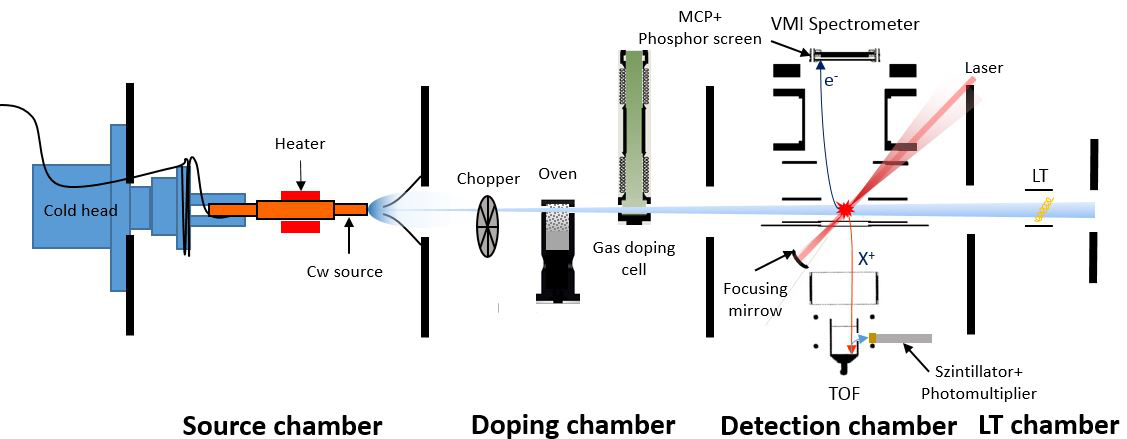
\includegraphics[width=16 cm]{../Images/setup.png}
\caption{Sketch of the vacuum chambers, including the main parts of the setup}
\end{figure}


\section{Source Chamber}

The Source chamber consists of a 6-way CF vacuum chamber, with a 2-stage cryostat which power a cold-head that can be cool down to 9K. It is located at the entrance of the chamber, parallel to the floor with an attached conical nozzle for the gas expansion process. The cooling capacity of the cryostat consists of a copper tube, into which pre-cooled helium is introduced. It can be adjusted by operating two heating resistors in combination with a sensor diode for temperature measurement and a PID controller. Controlling the resistor current the temperature at the end of the nozzle can be keeping it stable. The conical nozzle used to generate the atomic beam is the standard used in the research group on Nanoplasma research directed by Prof. Frank Steankeirmeyer at Freiburg University.  It is made of copper and has a platinum plate on front with a hole of 5$\mu m$ of diameter for $He$ experiments and 15$\mu m$ for $Ne$ gas clusters. The diameters were choose in order to follow the size dependence of the \textit{Hagenas} law, which together with the adjustable gas pressure and the nozzle temperature regulates the flow.
The cold head-nozzle arrangement are connected to the chamber via a self-made x-y manipulator,  with a thermally insulating rubber ring, which allows a beam adjustment in relation to the other components in the setup without breaking the vacuum. At the bottom of the chamber an Agilent turbo pump of $1800 L/s$ capacity is attached to a pre-vacuum scroll pump as exhaust.
A skimmer with a diameter of $400\mu m$ is located in front of the effusive jet, sorting the gas beam not just by size but also by its velocity vectors, allowing just those beams with direction along Z. To adjust the nozzle optimally to the skimmer, it is connected to an x-y displacement unit and can be aligned from outside the vacuum chamber. To prevent the small opening of the nozzle from clogging over time, high-purity helium 6.0 (99.9999$\%$ purity) and Ne 5.0 (99.999$\%$ purity) are used, this clean gas ensures a constant gas flow through the nozzle. At this extreme temperature any impurity in the gas bottle can condense, blocking the nozzle or changing the conditions of the clusters formation. 

\section{Doping Chamber}

As explained, the doping process takes place by inelastic impacts with atoms from the gas phase, referenced as the pick-up technique. In this experiment we doped with both metals and noble gases, and two different methods of doping are used: Metals are heated in evaporated phase in the oven, while gas dopant yield in a Gas doping cell entered the vacuum chamber through a needle valve. On the next section, we will explain the elements of the doping chamber and its most important characteristics used.

The oven chamber is connected after to the Source chamber via the skimmer, it is also a 6-way CF vacuum chamber, with a turbo pump on the bottom, connected to its own pre-vacuum scroll pump. On the sides the flanks allow a cold trap not used in this experiment, on the other side the flank that permit connection to the oven and the vacuum sensor. The Skimmer is made of Nickel, a very thin metal easy to bend, so in order to prevent strong pressure differences in the chamber that can modify the skimmer, a bypass is connected between the two chambers using a stainless steel flexible hose.  
An internal stand is welded to the front of the chamber and aligned with the skimmer. This stand supports the Chopper, the gas doping cell and the oven.
In the front the rail the choppers is located.  It is a steel  disk with three notches uniformed located, two photocells around the bottom of the disk reads the position of the bottom notches so the upper one can be positioned right in front the skimmer. In this way, when the disk rotates the beam can pass or its block by the disk in a controlled way.  

After the chopper, there is the Gas Doping cell, a circular flat metal base with a self-modified KF hose. The base of the cell has a matching pattern so the hose can be easily put and remove without losing the alignment. The stainless steel flexible hose has two $5mm$ hole (one in front and one opposite to it, some cm up the base) aligned to the skimmer so the gas bean can go though. The hose is fixed to the base and goes to the top of the chamber where it is connected to a "swagelok" needle valve that allows to control the gas flux for doping the beam. A Pfiffer CMR375 Capacitive sensor is located after the needle valve so a better control of the pressures and the number of dopant in the cluster. The bendable construction allows, not just to remove the doping cell without difficulty, but also to fit it on the top without depending on a fix way to locate the top plank, in this way there is room for maneuvering and the installation is faster.

Finally, at the end of the rail lies the Oven. As shown in fig \ref{img:oven} the oven consists of a patterned base (similar to the gas cell) that can  move a few $mm$ on $x-y$ plane. Over it, a metal cylinder with 4 heating cartridges holds a movable crucible in the center that contains the dopant sample, this movable container is set down by a rod that comes from the top of the chamber after a valve. Both, the stove and crucible have holes (a conical entrance of $40mm$ diameter and $3mm$ diameter respectively) that allows the pass of the gas beam and are aligned to the beam pad, in this way  the passing Atomic beam takes dopants via collisions with the vaporized sample material.

\begin{figure}[h!] 
\centering
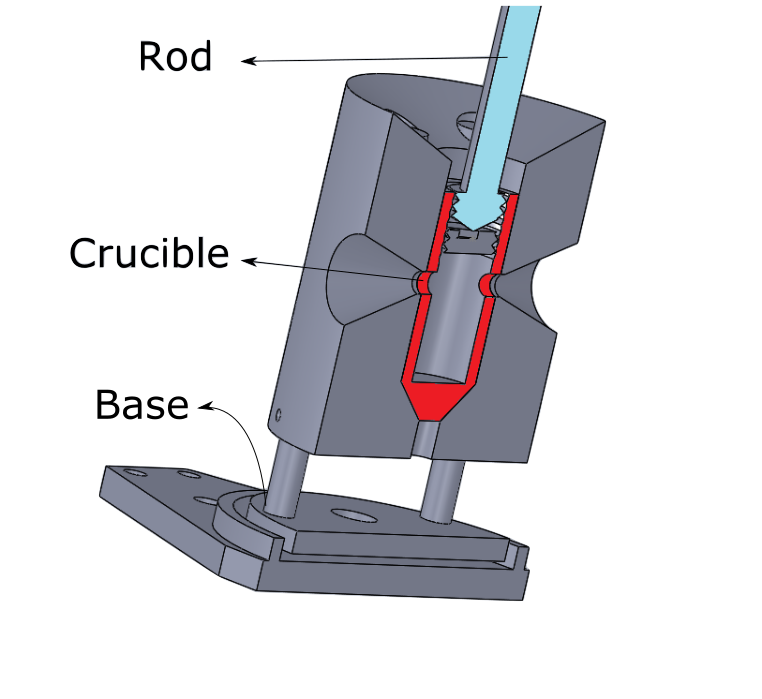
\includegraphics[width=8cm]{../Images/oven_complete_cut_2.PNG}
\caption{Cut of the Oven design, including part of the rod and the crucible.}
\label{img:oven}
\end{figure}

One important advantage of this new oven design done by \textit{Dominic Schomas},  is that the dopant can be change without braking the vacuum, it was tested in this experiment and prove to be useful in saving time and effort. To control the temperature of the oven a temp sensor is fixed in the stove, and the resistors current is manage by a PID controller allowing a stable temperature during the experiment. The maximal temperature reached was $450^{\circ}c$,  enough to create the gas phase for the potassium K and calcium Ca used in this experiment. Finally, there is an extra skimmer of diameter $2mm$, fixed to a valve between the connection of the doping chamber and the detection chamber that helps to avoid the disperse beams or an overflow from one chamber to the other.

In addition to the doped gas nano droplets, effusive gas is also released from the dopant chamber into the detector chambers through the needle valve and can be ionized and detected there. This disperse gas was pouring in directly on the chamber or filtered by diffused atoms going out of the oven and passing across the second skimmer once the choppers is close. This atomic gases were added for calibration of the detectors and background reduction allowing just one gas at a time.

\section{Detection chamber}

As mentioned, the detector chamber is connected to the Oven chamber through a valve and a skimmer. The detector chamber contains a newly developed Velocity-Map-Imaging
Spectrometer on top, a time-of-flight mass spectrometer on bottom and a LT detector in front. In this section we will give a brief presentation of the VMI and the TOF used for this experiment, taking special interest in the new Triggering process that allows to detect single nanoplasma explosions. 
 
 
\subsection{Velocity Map Imaging Spectrometer}

Velocity map imaging (VMI) is a widely used technique in areas such as atomic and molecular physics and physical chemistry. It is used to investigate velocity distributions of charged particles, which are generated in a defined volume, typically by photoionization.
A laser pulse generates charged particles by photoionization in the interaction region, which are accelerated by an electric field created by two electrodes.
The VMI used in this experiment is a modification on the original design by Eppink-Parker \cite{eppink_velocity_1997}. Its is made by a lower  electrode called Repeller followed by the extractor, ground electrodes which generated the electric filed that drives the particles to a detection system consisting of an Microchannel plate or MCP  and a Phosphor screen, which is observed by means of a CCD camera on top.  All electrodes have a circular layout and are about $1 mm$ thick.  The extractor and ground electrodes have a concentric hole where the particles pass through.
Once the Electron or Ions, guided by the electrodes, arrive to the MCP an electronic avalanche occurs, increasing the signal of each individual particle. The electronic avalanche hit the Phosphoscreen producing photons that can be detected with the camera focused on top.

\subsubsection{ Velocity distribution in VMI}

In order to describe the velocity distribution detected by the VMI, we assume that the charged particles come from a point in space emitted between the Repeller and the extractor. Furthermore, we presume that the initial kinetic energy of the particles obtained during the ionization process is small, in comparison to the energy supplied by the electric field.
The initial conditions of the charged particles are determined by the ionization volume and the initial velocity vectors $v_{i} = (v_{x};v_{y}$, whose distributions are of interest. The particles are drive by the Electric field in the direction $v_{z}$ to the spectrometer axis.
If one starts from an isotropic initial distribution for the velocities, particles with differing initial velocity vectors can finish in the same point on the detector, as shown in fig \ref{ing:vmiVelcDist}. This results in a loss of information, its is expected because we are trying to 3D information from a 2D projection.

\begin{figure}[h!]

\caption{Representation of particle trajectories A, B and C of the ionization volume to the detector plane, which, in spite of initially different velocity the finish on the same point of the detector plane. Withdrawn from \cite{fechner_lutz_aufbau_2011}}
\centering
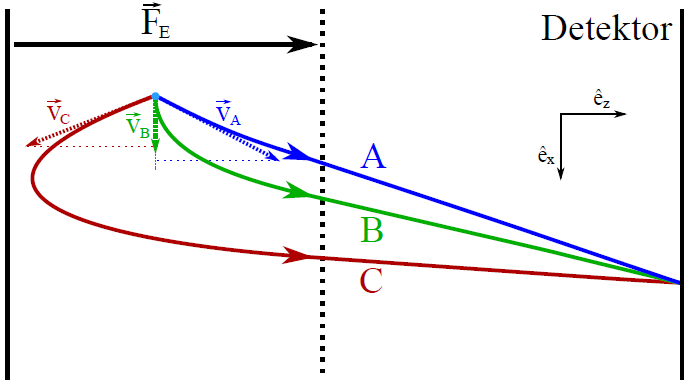
\includegraphics[width=8 cm]{../Images/cel distrub vmi.png}
\label{ing:vmiVelcDist}
\end{figure}

Assuming a cylindrically symmetric distribution $f(r,y)$ along the $y$-axis. If an infinitely far away observant look at the distribution $F$ along the $z$-direction.  With a basic axis conversion it can be shown that along the Z direction, the projection of the distribution $F$ of the integrated signal respond to.

\begin{equation}
F(x,y)=2\int^{\inf}_{\mid x\mid} \dfrac{f(r,y)r}{\sqrt{r^{2}-x^{2}}}*dr 
\end{equation}

Been F in cylindrical coordinates and $r^{2}=x^{2}+z^{2}$. Also called \textit{Abel-transform}.
But in order to resolve our signal we need the opposite procedure, turn this 2d distribution into the 3d spherical distribution that we assume in the beginning. For this process is called \textit{Inverse Abel-transform}, and it can be shown as.
 
\begin{equation}
F(r,y)=\dfrac{1}{\pi} \int^{\inf}_{\mid x\mid} \dfrac{dF(x,y)}{dx} \dfrac{1*dx}{\sqrt{r^{2}-x^{2}}} 
\end{equation}

The main problem that carries this transformation is that is not resolvable to a non-continues distribution that is the case of the Images recorded by the camera. So a numerical method needs to be used.
Fortunately, a Software Pbasex, is available to solve this integral. The idea is to have a basis function $f_{k}$ (in this case Lagrange polynomial ) in the space of distributions $f$.  Their projections $F_{k}$ onto the detector are well known, and the Able transform will be set as:

\begin{equation}
F_{k}(x) = 2\sigma \rho_{k}(x)\lbrace 1 + \sum^{k^{2}}_{1}\lbrace (x/\sigma)^{-2l} \prod^{l}_{m-1}(\dfrac{(k2+ 1-m)(m-1/2)}{m}\rbrace \rbrace
\end{equation}

If every measured image can be expressed on this basis, then the reconstruction of the F distribution when $k\rightarrow \inf$ can be obtained. A graphical example of this transformation is given in fig \ref{img:Abel} where each color represents a $f_{k}$ projection, where all $f$ are in the same basis, the sum of all the different $f$ will set the final reconstructed $F_{K}$.

\begin{figure}[h!]
\label{img:Abel}
 \caption{At the top of the graphic some basic functions $f_{k}$ in different colors, which can be used for the Inverse-Abel transform in the Basex method. On the bottom, the corresponding Abel-transformed functions Fk. Taken from \cite{fechner_lutz_aufbau_2011}}
 \centering
 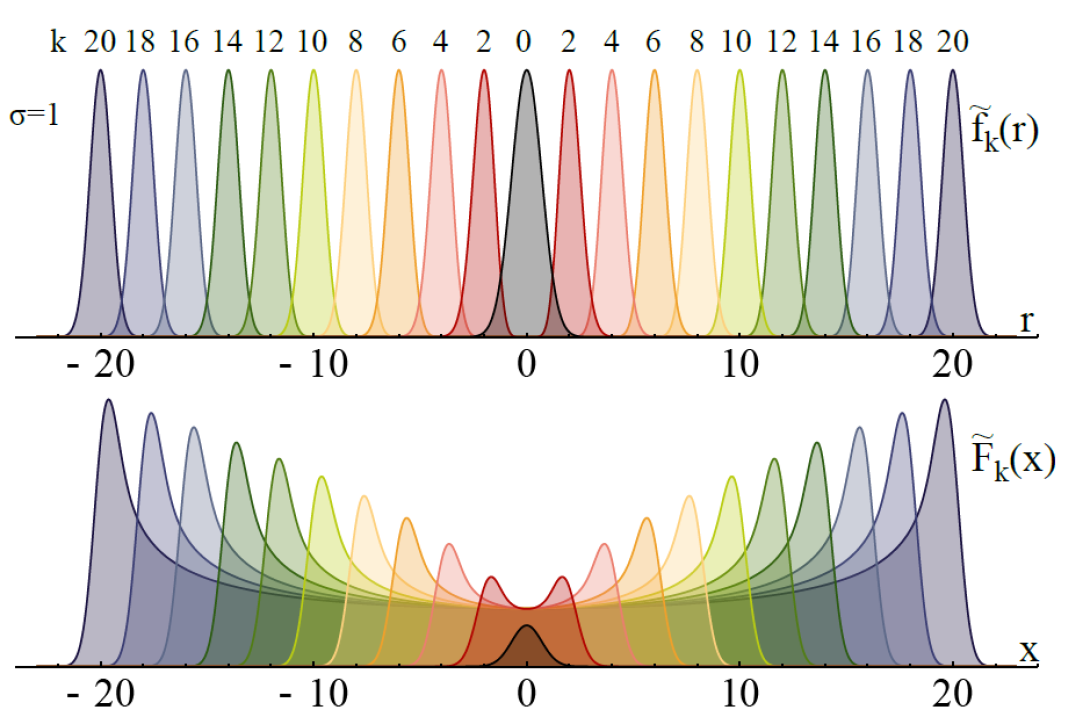
\includegraphics[width=10 cm]{../Images/abel transform pbasex function.png}
 \end{figure}


\subsubsection{VMI Parameters}

The VMI detector used in this experiment is detailed in \cite{schomas_compact_2017}, this construction basically follows the standard geometry of Eppink and Parker\cite{eppink_velocity_1997}. It is composed by three electro lenses (Repeller, lens and extractor) that focuses the ions or electrons on a $86,6mm$ (effective area) diameter Micro channel plates (MCP) arrange. This detector set is basically  two MCP`s superposed,  rotated to each other and a phosphoscreen (PS) layer of same diameter facing the top plank of the chamber with a Ca-fluoride glass of $1mm$ thick. An external CCD camera is focused to the PS. 

\begin{table}[]
\centering
\begin{tabular}{|l|l|l|l|}
\hline
\rowcolor[HTML]{EFEFEF} 
VMI & Repeler & Extractor & Lens  \\ \hline
X1  & -2430   & -1940     & 3500  \\ \hline
X3  & -7290   & 5820      & 10500 \\ \hline
Ion & 2430    & 1940      & 0     \\ \hline
\end{tabular}
\end{table}

The voltages applied to the MCP and PS determine the brightness of the final pictures of the ions, so in general just one set of voltages has been used, around $1400V$ for the MCP and $4000V$ for the Ps. The achievable energy acceptance for this stack is $34eV$ for a the VMI setting 1 and $270 eV$ for the X3 settings. The VMNI have a resolution of $\bigtriangleup E / E\leq 4\%$ \cite{schomas_compact_2017}. The camera used in the experiment was a Basler acA1920-155um focused on the PS.

\begin{figure}[hbtp]
\label{img:mcp cut}
\centering
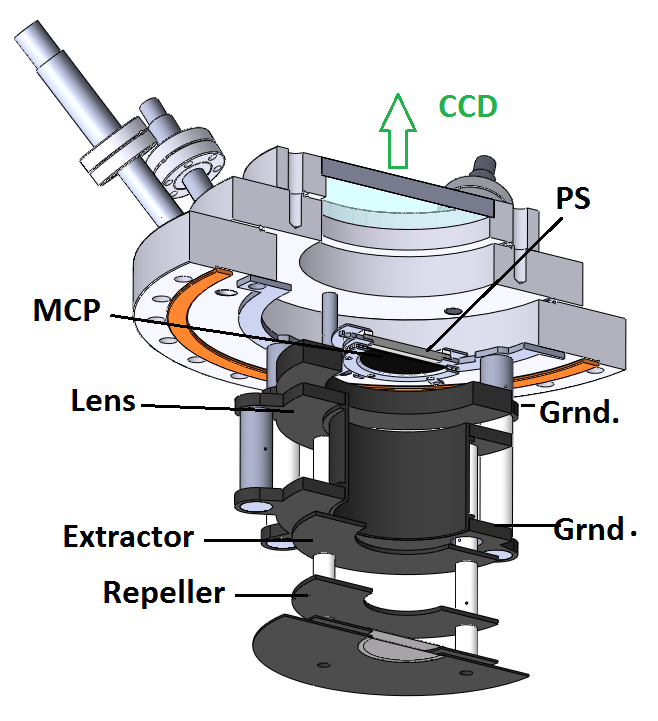
\includegraphics[width =8 cm]{../Images/MCP cut.png}
\caption[MCP sketch cut]{Sectional cut view of the CAD model of the spectrometer setup. On black, the electrodes and the white the Polyether ketone (PEEK) isolators. On orange, the cooper ring and on blue the top window facing the CCD camera
}
\end{figure}

On fig \ref{img:mcp cut} we present a view of the model of the VMI used in this experiment, From bottom to top, the structure of the electrodes consists of two Repeller electrodes separated by a few millimetres with circular openings on which a fine mesh copper grid is applied, an aperture electrode as Extractor, another aperture electrode which is held at ground potential and then from the extended lens electrode with the following second ground electrode. At the top, the MCP-PS arrange (on black the MCP and on gray the PS) facing the center of the window installed in the top plank of the chamber. Around the window there are three connections that allow the voltages for the electrodes and the cables are carefully arranged around the structure to avoid discharges or even disturb the uniform electric field.

The openings of the Repeller (at the bottom in bluish color) electrodes allow the use of these electrodes as well as extractor electrodes for a TOF spectrometer. In simultaneous operation of the VMI and the TOF spectrometer, the glued grids prevent mutual field effects of the two spectrometers.  The Repeller and extractor are grade 2 titanium and the lens is stainless.

\subsection{Time of Flight Spectrometer}

The Time of flight (TOF) spectrometer used was based on the design by Wiley and McLaren \cite{wiley_timeflight_1955}. As its name refers, the TOF mass spectrometer relates the time that a particle at an electric field requires to reach certain distance with its mass, when atoms and molecules are photoionized,  they pass through an electrostatic acceleration field and are registered in a detector after crossing a field-free flight path. Based on the flight time the ratio $m/q$ of a particle can be determined as:

\begin{equation}
t-t_{0}=a\sqrt{\frac{m}{q}}
\end{equation}

Where $a$ is an experimental factor depending of the flight distance, electric fields and material of the setup,  $m/q$ is the relation mass - charge, $t_{0}$ is the time ionization time (given by the laser )and $t$ is the time of flight.

The ions creation takes place in the aperture between the Repeller and extractor electrodes. Behind the extractor electrode there is a further aperture electrode, which is held at zero potential and thus generates a pre establish flight route with a defined field, grids are glued to the openings of the electrodes to prevent the propagation of the fields through the orifices in the electrodes. The Repeller electrode is set to a positive potential and the extractor to a negative potential. The resulting electric field accelerates the ions through the openings in the flight tube, on which grids mount on both sides keep the drift path free of field.
Once the coulomb explosion takes place, the ions are accelerated by the electric field of the Repeller and then fly through a field-free drift path to the detector. This allows a complete mass spectrum to be recorded within a few microseconds in a single measuring step \cite{mobius_time--flight_2016}.

\begin{figure}[hbtp]
\label{img:tofcup}
\centering
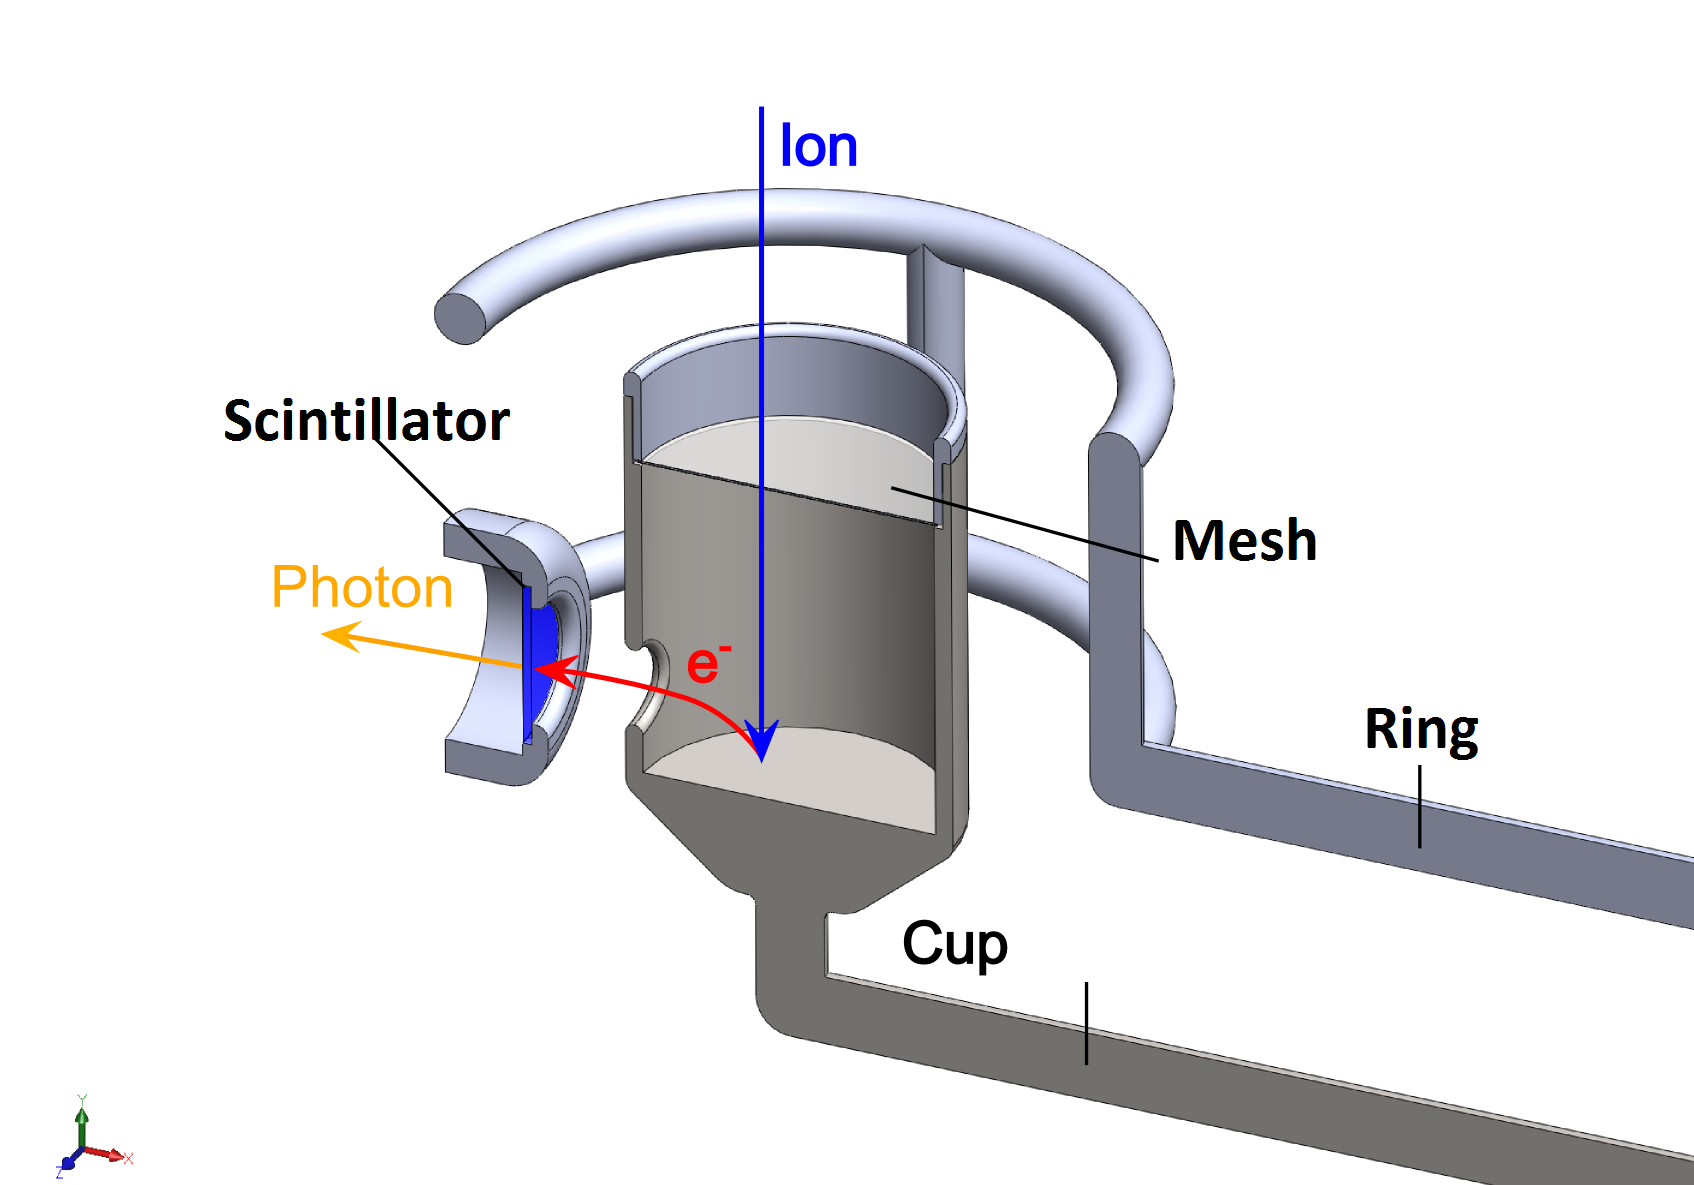
\includegraphics[width = 10 cm]{../Images/Cup scintillator.png}
\caption[TOF cup]{Illustration of the functional principle of a Daly detector.}
\end{figure}

The flying Ions finally are detected by a Daly detector \cite{daly_scintillation_1960}. It consists of a cup, a grid and a ring. The cup lies on negative high voltage while the ring for positive. The ions from the Repeller pass through the field free tube corrected by a drift electrode.  Since in the direction of the hole the potential for electrons drops sharply, the ring electrode generates an electric field, which directs the ions into the cup. The ions that pass the grid at high speed hits on the bottom of the cup, they generate some electrons, which are transmitted through a small hole in the bottom and then in a scintillator Eljen technology (EJ-204) flashes some photons in the process. These light is detected in a Hammamatzu r-647 photomultiplier (PM). The voltage output of the PM is controlled by a fast analogue-to-digital converter, and it is used at $900V$ voltage. The cup and the drift-scintellator  tube was set at high voltages,  $-17000V$ and $-4000$ respectively.

\subsection{LT Detector}

The Langmuir-Taylor detector (LT detector) chamber consists of a small CF40-6-way chamber. The detector consists essentially of an annealing filament, which is located between two planar round electrodes. The Operating Principle of an LT-Detector is based on surface ionization by the tunnel effect \cite{delhuille_optimization_2002}. For the annealing filament is typically used  rhenium, platinum or tungsten, as this is the most common due its comparatively high electron work function. With high voltages, the wire reaches high temperatures, as a consequence, a passing neutral atom is ionized, releasing an electron into the wire. The resulting ions are attracted by the negative electrodes around the wire generating a current. The ionic current generated at the electrodes is proportional to the number of ionized atoms and is measured using a picoammeter.
The LT chamber is connected to the VMI chamber via an orifice plate and is used mainly as a beam dump and to align the detector. The most current generated in the chamber the most atoms are passing through the hole, so we can be sure that the beam pad is in the detection area.

